% !TEX TS-program = pdflatex
% !TEX encoding = UTF-8 Unicode

% This is a simple template for a LaTeX document using the "article" class.
% See "book", "report", "letter" for other types of document.

\documentclass[11pt]{report} % use larger type; default would be 10pt

\usepackage[utf8]{inputenc} % set input encoding (not needed with XeLaTeX)

%%% Examples of Article customizations
% These packages are optional, depending whether you want the features they provide.
% See the LaTeX Companion or other references for full information.

%%% PAGE DIMENSIONS
\usepackage{geometry} % to change the page dimensions
\geometry{a4paper} % or letterpaper (US) or a5paper or....
% \geometry{margin=2in} % for example, change the margins to 2 inches all round
% \geometry{landscape} % set up the page for landscape
%   read geometry.pdf for detailed page layout information

\usepackage{graphicx} % support the \includegraphics command and options

% \usepackage[parfill]{parskip} % Activate to begin paragraphs with an empty line rather than an indent

%%% PACKAGES
\usepackage{booktabs} % for much better looking tables
\usepackage{array} % for better arrays (eg matrices) in maths
\usepackage{paralist} % very flexible & customisable lists (eg. enumerate/itemize, etc.)
\usepackage{verbatim} % adds environment for commenting out blocks of text & for better verbatim
\usepackage{subfig} % make it possible to include more than one captioned figure/table in a single float
% These packages are all incorporated in the memoir class to one degree or another...

%%% HEADERS & FOOTERS
\usepackage{fancyhdr} % This should be set AFTER setting up the page geometry
\pagestyle{fancy} % options: empty , plain , fancy
\renewcommand{\headrulewidth}{0pt} % customise the layout...
\lhead{}\chead{}\rhead{}
\lfoot{}\cfoot{\thepage}\rfoot{}

%%% SECTION TITLE APPEARANCE
\usepackage{sectsty}
\allsectionsfont{\sffamily\mdseries\upshape} % (See the fntguide.pdf for font help)
% (This matches ConTeXt defaults)

%%% ToC (table of contents) APPEARANCE
\usepackage[nottoc,notlof,notlot]{tocbibind} % Put the bibliography in the ToC
\usepackage[titles,subfigure]{tocloft} % Alter the style of the Table of Contents
\renewcommand{\cftsecfont}{\rmfamily\mdseries\upshape}
\renewcommand{\cftsecpagefont}{\rmfamily\mdseries\upshape} % No bold!

\usepackage[hidelinks]{hyperref}
\usepackage{float}

\usepackage[italian]{babel}

\usepackage{biblatex} %Imports biblatex package
\bibliography{citations} %Import the bibliography file

\setlength{\parindent}{0cm}

\usepackage{listings}
\usepackage{color}
\definecolor{lightgray}{rgb}{.9,.9,.9}
\definecolor{darkgray}{rgb}{.4,.4,.4}
\definecolor{purple}{rgb}{0.65, 0.12, 0.82}

\lstdefinelanguage{SWRL}{
  keywords={},
  otherkeywords={^, ->},
  keywordstyle=\color{blue}\bfseries,
  identifierstyle=\color{black},
  sensitive=false,
  breakatwhitespace=true
}

\lstset{
   backgroundcolor=\color{lightgray},
   extendedchars=true,
   basicstyle=\footnotesize\ttfamily,
   showstringspaces=false,
   showspaces=false,
   numbers=none,
   tabsize=2,
   breaklines=true,
   showtabs=false,
   captionpos=b
}

\usepackage{graphicx}
\graphicspath{ {./} }

%%% END Article customizations

%%% The "real" document content comes below...

\title{FootOntologyPlus}
\author{The Author}
\author{The Authors}
\date{} % Activate to display a given date or no date (if empty),
         % otherwise the current date is printed 

\begin{document}
\maketitle

\newpage

\renewcommand*\contentsname{Indice}

\tableofcontents
\newpage

\chapter{Introduzione}

Citazione \cite{test}

\chapter{Ontologia di partenza}

\chapter{Modifiche all'ontologia}

\chapter{Inserimento di individui}

\chapter{Regole SWRL}

\textbf{SWRL} (\textbf{Semantic Web Rule Language}) è un linguaggio usato nell'ambito del Semantic Web per esprimere regole di inferenza e vincoli logici più complessi di quelli realizzabili usando il solo OWL.

\hfill

Nella nostra ontologia abbiamo inserito numerose regole, utili a:

\begin{enumerate}
    \item inferire nuovi collegamenti tra i dati
    \item individuare casi di errore sui dati
\end{enumerate}

Le sezioni che seguono riportano tali regole, non in un ordine particolare.

\section{HomeFormationRule}

Questa regola "raffina" il collegamento tra una formazione e una partita, esplicitando che la prima è usata dalla squadra in casa.
Questo perché \texttt{isAwayFormationIn} è una sottoproprietà di \texttt{isFormationIn}.

\begin{lstlisting}[language=SWRL]
isHomeTeam(?t, ?m) ^ hasFormation(?t, ?f) ^ isFormationIn(?f, ?m) -> isHomeFormationIn(?f, ?m)
\end{lstlisting}

\section{AwayFormationRule}

Questa regola funziona in modo analogo alla precedente, ma riguardo la squadra in trasferta.

\begin{lstlisting}[language=SWRL]
isAwayTeam(?t, ?m) ^ hasFormation(?t, ?f) ^ isFormationIn(?f, ?m) -> isAwayFormationIn(?f, ?m)
\end{lstlisting}

\newpage

\section{DuplicateSubstituteRule}

Questa regola verifica se un giocatore segnato come riserva partecipa a multiple sostituzioni come giocatore entrante, e in tale caso gli assegna una classe di errore.

\begin{lstlisting}[language=SWRL]
hasReservePlayer(?f, ?p) ^ hasEnteringPlayer(?s1, ?p) ^ hasEnteringPlayer(?s2, ?p) ^ differentFrom(?s1, ?s2) ^ hasTeamFormation(?m, ?f) ^ hasSubstitution(?m, ?s1) ^ hasSubstitution(?m, ?s2) -> DuplicateSubstituteError(?p)
\end{lstlisting}

\section{DuplicateSubstitutedRule}

Il funzionamento di questa regola è analogo alla precedente, ma riguardante il giocatore uscente.
Questa regola copre però solo i giocatori titolari (ovvero i giocatori che partecipano alla partita dall'inizio).

\begin{lstlisting}[language=SWRL]
hasStarterPlayer(?f, ?p) ^ hasExitingPlayer(?s1, ?p) ^ hasExitingPlayer(?s2, ?p) ^ differentFrom(?s1, ?s2) ^ hasTeamFormation(?m, ?f) ^ hasSubstitution(?m, ?s1) ^ hasSubstitution(?m, ?s2) -> DuplicateSubstitutedError(?p)
\end{lstlisting}

\section{StarterAsSubstituteRule}

Questa regola verifica se un giocatore titolare è il giocatore entrante in una sostituzione, e in tale caso gli assegna una classe di errore.

\begin{lstlisting}[language=SWRL]
hasStarterPlayer(?f, ?p) ^ hasEnteringPlayer(?s, ?p) ^ hasTeamFormation(?m, ?t) ^ hasSubstitution(?m, ?s) -> StarterAsSubstituteError(?p)
\end{lstlisting}

\section{FriendlyMatchInTournamentRule}

Non è corretto assegnare una partita amichevole ad un torneo, qualsiasi sia il suo tipo, e se ciò viene fatto allora una classe di errore è assegnata alla partita. 

\begin{lstlisting}[language=SWRL]
includedInTournament(?m, ?t) ^ FriendlyMatch(?m) -> FriendlyMatchInTournamentError(?m)
\end{lstlisting}

\section{GoalScoredByTeamRule}

Questa regola collega un goal ad una squadra, sapendo che il goal è stato fatto da un giocatore che giocava in tale squadra nella partita.

\begin{lstlisting}[language=SWRL]
scores(?p, ?g) ^ hasEvent(?m, ?g) ^ isPlayerInFormation(?p, ?f) ^ hasFormation(?t, ?f) ^ competesIn(?t, ?m) -> scoredByTeam(?g, ?t)
\end{lstlisting}

\section{InconsistentBallPossessionInMatchRule}

Questa regola controlla se la somma del possesso palla indicata nelle statistiche di performance per le squadre che hanno giocato una partita non è 100\%, e in tale caso assegna una classe di errore alla partita e alle statistiche.

\begin{lstlisting}[language=SWRL]
teamStatsIn(?ps1, ?m) ^ teamStatsIn(?ps2, ?m) ^ differentFrom(?ps1, ?ps2) ^ BallPossession(?ps1, ?p1) ^ BallPossession(?ps2, ?p2) ^ swrlb:add(?r, ?p1, ?p2) ^ swrlb:notEqual(?r, 100) -> InconsistentBallPossessionInMatchError(?m) ^ InconsistentBallPossessionInMatchError(?ps1) ^ InconsistentBallPossessionInMatchError(?ps2)
\end{lstlisting}

\section{InconsistentContractDatesRule}

Questa regola verifica se le date di un contratto sono inconsistenti (data di inizio futura alla data di fine).

\begin{lstlisting}[language=SWRL]
ContractStartDate(?c, ?sd) ^ ContractEndDate(?c, ?ed) ^ temporal:before(?ed, ?sd) -> InconsistentContractDatesError(?c)
\end{lstlisting}

\section{InconsistentMatchScoresHome/AwayRule}

Queste due regole verificano se il vincitore di una partita non è consistente con i punteggi assegnati alle due squadre.
Sono state necessarie due regole in quanto i punteggi delle squadre sono legati alla partita e non direttamente alle squadre.

\begin{lstlisting}[language=SWRL]
isHomeTeam(?t1, ?m) ^ isAwayTeam(?t2, ?m) ^ hasWinner(?m, ?t1) ^ MatchHomeTeamScore(?m, ?s1) ^ MatchAwayTeamScore(?m, ?s2) ^ swrlb:lessThanOrEqual(?s1, ?s2) -> InconsistentMatchScoresError(?m)
\end{lstlisting}

\begin{lstlisting}[language=SWRL]
isHomeTeam(?t1, ?m) ^ isAwayTeam(?t2, ?m) ^ hasWinner(?m, ?t2) ^ MatchHomeTeamScore(?m, ?s1) ^ MatchAwayTeamScore(?m, ?s2) ^ swrlb:lessThanOrEqual(?s2, ?s1) -> InconsistentMatchScoresError(?m)
\end{lstlisting}

\section{InvalidLeagueMatchFormatExtraTime/PenaltyRule}

Le partite che fanno parte di una lega non possono avere supplementari o rigori, e queste due regole servono a identificare tali inconsistenze.

\begin{lstlisting}[language=SWRL]
includedInTournament(?m, ?t) ^ League(?t) ^ ExtraTimePlayed(?m, true) -> InvalidLeagueMatchFormatError(?m)
\end{lstlisting}

\begin{lstlisting}[language=SWRL]
includedInTournament(?m, ?t) ^ League(?t) ^ PenaltyShootoutPlayed(?m, true) -> InvalidLeagueMatchFormatError(?m)
\end{lstlisting}

\section{InvalidMatchRule}

Questa regola verifica se una squadra sta giocando contro sé stessa in una partita.

\begin{lstlisting}[language=SWRL]
hasHomeTeam(?m, ?t) ^ hasAwayTeam(?m, ?t) -> InvalidMatchError(?m)
\end{lstlisting}

\section{MultipleRedCardsRule}

Questa regola controlla se un giocatore ha ricevuto multipli cartellini rossi in una partita.

\begin{lstlisting}[language=SWRL]
hasReceived(?p, ?c1) ^ hasReceived(?p, ?c2) ^ RedCard(?c1) ^ RedCard(?c2) ^ differentFrom(?c1, ?c2) ^ hasEvent(?m, ?c1) ^ hasEvent(?m, ?c2) -> MultipleRedCardsError(?p)
\end{lstlisting}

\section{NonGoalKeeperWithSavesRule}

Questa regola verifica se le statistiche di un giocatore indicano il numero di parate sebbene esso non abbia giocato come portiere nella partita.

\begin{lstlisting}[language=SWRL]
playsInPosition(?pl, ?p) ^ Outfield(?p) ^ hasPlayerStats(?pl, ?ps) ^ Saves(?ps, ?s) ^ hasPlayer(?m, ?p) ^ hasPlayerPerformanceStats(?m, ?ps) -> NonGoalKeeperWithSavesError(?pl)
\end{lstlisting}

\section{PlayerInMatchRule}

Questa regola collega un giocatore ad una partita, sapendo che il giocatore era in una formazione utilizzata in tale partita.

\begin{lstlisting}[language=SWRL]
hasPlayerInFormation(?f, ?p) ^ isFormationIn(?f, ?m) -> hasPlayer(?m, ?p)
\end{lstlisting}

\section{TeamNotInMatchRule}

Questa regola controlla se un evento in una partita è legato ad una squadra che non gioca in tale partita.

\begin{lstlisting}[language=SWRL]
hasEvent(?m, ?e) ^ hasMatchEvent(?t, ?e) ^ isHomeTeam(?t1, ?m) ^ isAwayTeam(?t2, ?m) ^ differentFrom(?t, ?t1) ^ differentFrom(?t, ?t2) -> TeamNotInMatchError(?t)
\end{lstlisting}

\newpage

\section{UncontractedPlayerInMatchRule}

Questa regola verifica se un giocatore ha partecipato ad una partita senza far parte di una delle due squadre coinvolte, in quanto non si trovava sotto contratto con una delle due squadre al momento della partita.
La regola copre soltanto i casi in cui il giocatore si trovava sotto contratto con un'altra squadra e se il contratto è terminato.

\begin{lstlisting}[language=SWRL]
signs(?t1, ?c) ^ involvesPlayer(?c, ?p) ^ participatesIn(?p, ?m) ^ includes(?m, ?t2) ^ includes(?m, ?t3) ^ differentFrom(?t1, ?t2) ^ differentFrom(?t1, ?t3) ^ ContractStartDate(?c, ?sd) ^ ContractEndDate(?c, ?ed) ^ MatchDate(?m, ?d) ^ temporal:before(?sd, ?d) ^ temporal:after(?ed, ?d) -> UncontractedPlayerInMatchError(?p)
\end{lstlisting}

\chapter{Interrogazioni SPARQL}

L'ultima parte del progetto è stata la realizzazione di interrogazioni usando \textbf{SPARQL} (\textbf{SPARQL Protocol and RDF Query Language}), un linguaggio simile a SQL per poter estrarre dati dall'ontologia.

\hfill

Le interrogazioni che abbiamo scritto sono esempi che producono risultati sulla base degli individui d'esempio che abbiamo predisposto. 
Per realizzarle abbiamo usato le viste \textbf{SPARQL Query} e \textbf{Snap SPARQL Query} di Protegé. 

\section{Interrogazione sui contratti di un giocatore}

Questa interrogazione recupera i contratti firmati da un giocatore (nell'esempio \texttt{Player1}) e i nomi dei team per cui i contratti sono stati firmati. 

\begin{lstlisting}
PREFIX : <http://visualdataweb.org/FootOntologyPlus/>

SELECT ?contract ?teamName
WHERE { 
    ?team :signsPlayer ?contract ;
          :TeamName ?teamName .
    ?contract :involvesPlayer :Player1 .
}
\end{lstlisting}

\begin{figure}[H]
	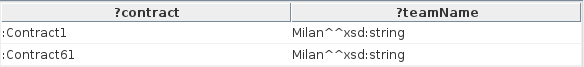
\includegraphics[width=\textwidth]{query1}
	\caption{Risultato della query sulla nostra ontologia.}
\end{figure}

\newpage

\section{Interrogazione sui contratti non terminati}

Questa interrogazione recupera tutti i contratti che non hanno una data di terminazione. Si assume in questo caso che tali contratti siano ancora attivi, ma in generale vige la "Open World assumption" riguardo alle informazioni mancanti.

\begin{lstlisting}
PREFIX : <http://visualdataweb.org/FootOntologyPlus/>

SELECT ?player ?team ?contract ?startDate
WHERE { 
    ?contract :isSignedForPlayerBy ?team ;
        :involvesPlayer ?player ;
        :ContractStartDate ?startDate .
    FILTER NOT EXISTS { ?contract :ContractEndDate ?endDate }
}
ORDER BY ASC (?player)
\end{lstlisting}

\begin{figure}[H]
	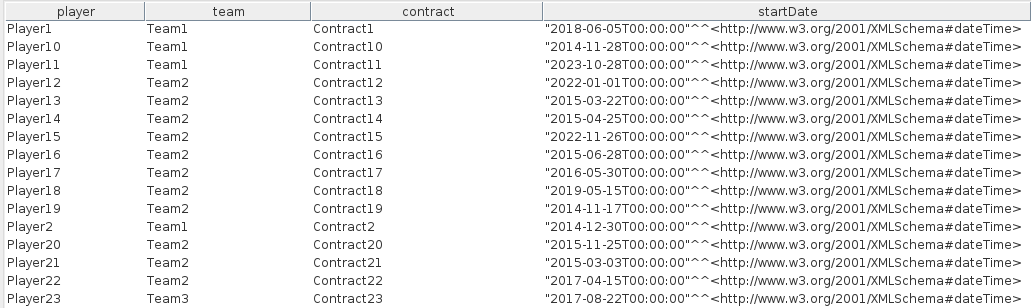
\includegraphics[width=\textwidth]{query2}
	\caption{Parte del risultato della query sulla nostra ontologia.}
\end{figure}

\section{Interrogazione sui cartellini ricevuti dai giocatori}

Questa interrogazione recupera le informazioni riguardanti i cartellini ricevuti dai giocatori, nello specifico il tipo di cartellino, la partita e il minuto di gioco in cui è stato ricevuto. 

\begin{lstlisting}
PREFIX rdf: <http://www.w3.org/1999/02/22-rdf-syntax-ns#>
PREFIX rdfs: <http://www.w3.org/2000/01/rdf-schema#>
PREFIX : <http://visualdataweb.org/FootOntologyPlus/>

SELECT ?player ?cardType ?match ?minute
WHERE {
    ?player :hasReceived ?card .
    ?card :MinuteOfEvent ?minute ;
        :isEventIn ?match ;
        rdf:type ?cardType .
    ?cardType rdfs:subClassOf :Card .
    FILTER (?cardType != :Card) .
}
ORDER BY ASC (?player)
\end{lstlisting}

\begin{figure}[H]
	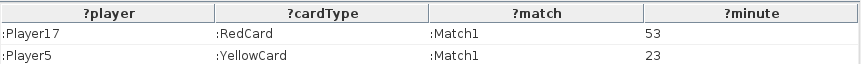
\includegraphics[width=\textwidth]{query3}
	\caption{Risultato della query sulla nostra ontologia.}
\end{figure}

\section{Interrogazione sulle sostituzioni effettuate in una partita}

Questa interrogazione le informazioni riguardanti le sostituzioni effettuate in una partita (nell'esempio \texttt{Match1}), nello specifico il nome dei giocatori coinvolti e il minuto di gioco. 

\begin{lstlisting}
PREFIX : <http://visualdataweb.org/FootOntologyPlus/>

SELECT ?enteringName ?exitingName ?minute
WHERE {
    ?sub :isSubstitutionIn :Match1 ;
        :hasEnteringPlayer ?entering ;
        :hasExitingPlayer ?exiting ;
        :MinuteOfEvent ?minute .
    ?entering :FullName ?enteringName .
    ?exiting :FullName ?exitingName .
}
ORDER BY ASC (?minute)
\end{lstlisting}

\begin{figure}[H]
	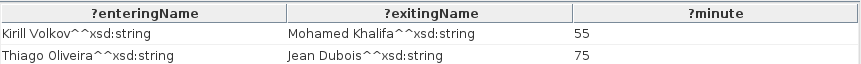
\includegraphics[width=\textwidth]{query4}
	\caption{Risultato della query sulla nostra ontologia.}
\end{figure}

\section{Interrogazione sui goal segnati dai giocatori}

Questa interrogazione recupera il numero di goal segnati da ogni giocatore in un torneo (nell'esemptio \texttt{League1}).

\begin{lstlisting}
PREFIX : <http://visualdataweb.org/FootOntologyPlus/>

SELECT ?player ?playerName (COUNT(?goal) as ?totalGoals) 
WHERE {
    ?match :includedInTournament :League1 ;
        :hasGoal ?goal .
    ?goal :scoredByPlayer ?player .
    ?player :FullName ?playerName
}
GROUP BY ?player ?playerName
ORDER BY DESC (?totalGoals)
\end{lstlisting}

\begin{figure}[H]
	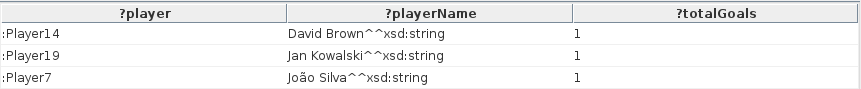
\includegraphics[width=\textwidth]{query5}
	\caption{Risultato della query sulla nostra ontologia. Il nome dell'individuo giocatore è incluso in caso di omonimi.}
\end{figure}



\chapter{Conclusioni}

\medspace

\printbibliography

\end{document}
